\section{Overview}
This supplement describes AIMI's runtime and training, followed by visual exploration (Q3), control during reasoning (Q2), complete-system comparisons (Q1), and pose estimation and hardware transfer (Q4). Q2 uses exactly three evaluation seeds, 187102, 187103 and 187104, with 40 trials per method and seed. Other seeds belong to separate studies or training diagnostics. Each result retains its study-specific denominator. Q4 includes 240 physical-hand trials on a cube, die, ball and duck; per-object counts are reported below. Recorded physical-hand image sequences remain to be added.

\section{Task and Runtime}
This section describes the cube system. The die, additional-object and language sections explain the differences for other objects.
\subsection{Object and goals}
Language-guided exploration seeks evidence for a requested surface target. Inspection changes the view; target binding associates the identified surface with a motor goal. Table~\ref{tab:mapping} records the cube's fixed face mapping. Body normals include the original mesh rotation. All methods use this mapping and the same cached six-vector bank. Cyan appears pale blue and magenta appears purple. The target quaternion specifies the reference orientation used for scoring.

\begin{table}[h]
\centering\small
\begin{tabular}{llcc}
\toprule
Letter & Skill color & Body normal & Target XYZW\\
\midrule
T & red & $(0,-1,0)$ & $(-s,0,0,s)$\\
E & green & $(-1,0,0)$ & $(0,s,0,s)$\\
R & blue & $(0,0,-1)$ & $(1,0,0,0)$\\
L & yellow & $(0,0,1)$ & $(0,0,0,1)$\\
S & magenta & $(0,1,0)$ & $(s,0,0,s)$\\
H & cyan & $(1,0,0)$ & $(0,-s,0,s)$\\
\bottomrule
\end{tabular}
\caption{Frozen goal mapping, with $s=\sqrt{1/2}$.}
\label{tab:mapping}
\end{table}

The instruction names a letter, and the benchmark checks its fixed reference orientation with a 0.16-radian tolerance. A drop ends the trial when the object moves at least 0.24 metres from its nominal grasp position. This rule does not detect every brief slip or loss of contact within that boundary.

\subsection{Physics and perception}
The runtime uses Isaac Lab 3.0, Isaac Sim 6.2, Newton 1.6.1, Warp 1.17, and PyTorch 2.11 with CUDA 13.0. The collision model contains 23 bodies and 117 shapes: 116 convex shapes and one box. Contact allocation uses \texttt{nconmax=4096} and \texttt{njmax=1024}. Runs with contact overflow are excluded from the reported experiments.

The frozen pose estimator predicts 27 image-coordinate/depth values for nine points and recovers pose through calibrated geometry. Its $120\times120$ rendered input includes live hand occlusion. Sensor calibration, object asset, policy normalization, joint order, action mapping and smoothing remain fixed within each study. The simulation pose results do not establish accuracy on real-camera images or unseen scenes.

\subsection{Timing, termination, and exclusions}
Each episode lasts at most 120 seconds of simulated control time. A model call taking $L$ wall-clock seconds must remain pending for at least $\lceil30L\rceil$ control steps, and its reply cannot be used before the call finishes. Physics continues throughout. Since simulation runs slower than real time, an episode takes longer in wall-clock time. Hardware control speed must be measured separately.

The stopping check runs at 3~Hz. The requested symbol must be bound to a goal, with no inspection or model request underway, and estimated orientation error must be at most 0.16 radians. The independent scorer then checks the actual requested face and true orientation using the same tolerance. It scores the stop time, without an extra holding period or credit for a better pose reached earlier.

A service error or model call exceeding 120 seconds is recorded without replacement. The original three-system panel removes trial 183102011 from every arm. This leaves 39 common eligible trials for that historical Q1 panel. The current Q2 study reports all 120 outcomes per method. Raw 40-trial outcomes remain visible, including service-affected cases.

\section{Models and Training}
Figure~\ref{fig:method-supp} expands the cube's deployed observation, goal-selection and control loop. The training procedures are described below.
\begin{figure*}[t]
\centering
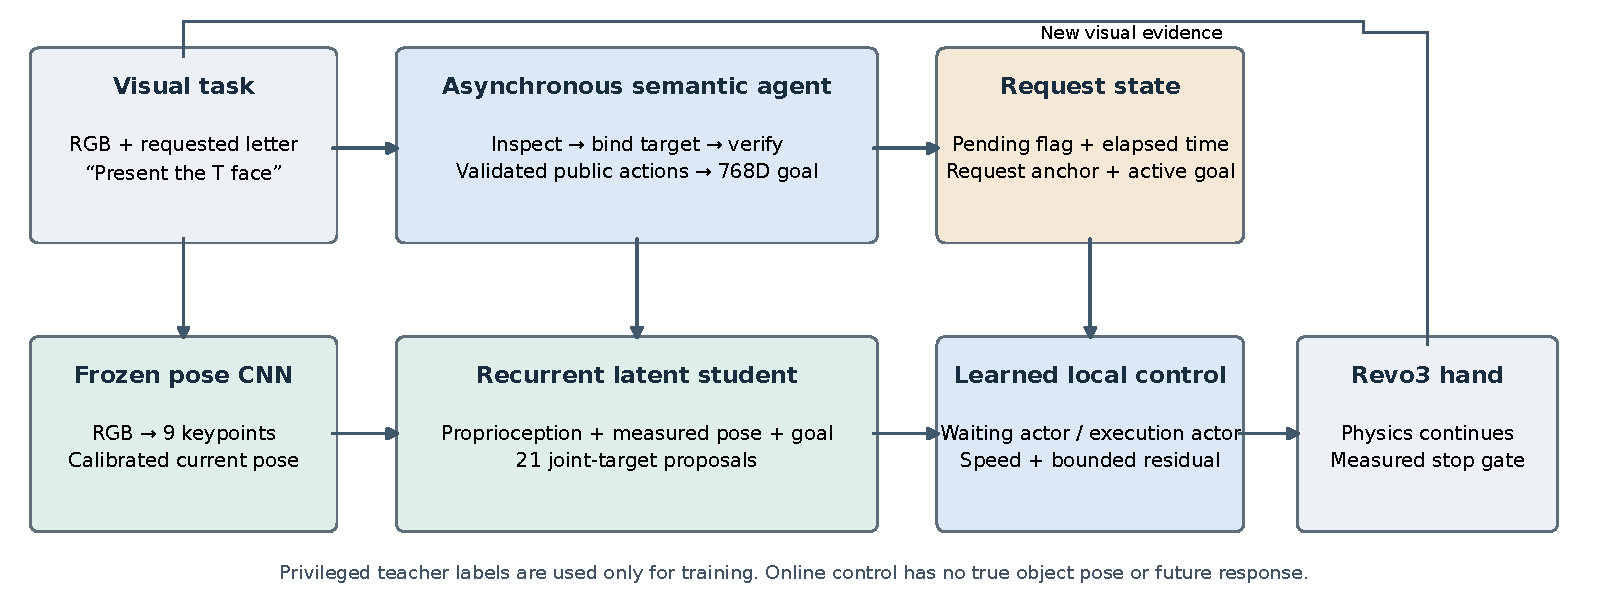
\includegraphics[width=.96\textwidth]{figures/method.pdf}
\caption{\textbf{Cube deployment loop.} An asynchronous agent selects motor goals from visual evidence. The pose estimator, student and local controllers continue operating between agent replies. Privileged teacher supervision is used only during training. This is a system schematic.}
\label{fig:method-supp}
\end{figure*}
\subsection{ViserDex-based Revo3 foundation and student adaptation}
Our motor foundation adapts ViserDex's teacher--student approach~\cite{bhardwaj2026viserdex} to the Revo3 hand. AIMI starts from the resulting pretrained teacher and student. The teacher remains frozen while the student learns its goal-bank interface. We reuse compatible observation encoders, recurrent and actor weights, and normalization statistics. The adapted student receives neither the target quaternion nor the relative-goal quaternion at deployment.

The student is fitted on collected trajectories using frozen-teacher action labels. Goal-projection warmup uses action MSE. Recurrent adaptation additionally uses a training-only decoder with normalized privileged state targets, excluding goal-quaternion channels; its reconstruction MSE has weight 0.2. The decoder provides auxiliary supervision and is absent from deployed control. This loss is distinct from the local-controller loss in the main paper.

\subsection{Semantic and motor inputs}
The motor policy receives 109 target-free proprioceptive/history features, seven measured pose values, and a 768-dimensional goal. Its goal projection has width 64 and a tanh nonlinearity. The inherited recurrent policy emits 21 normalized joint targets. The asset-specific goal quaternion is absent from the migrated student's inference inputs.

The hosted model route recorded in the experiment manifests is \texttt{gpt-6-astra}; the local grounding backbone is Qwen3-VL-4B-Instruct. AIMI passes validated tool arguments through a fixed goal-bank lookup. The fine-tuned baseline predicts a continuous vector within the normalized skill span. Neither receives the requested face's true pose. When the view is unreadable, the local baselines follow schedule $(1,3,0,2,4,5)$ with 90-step inspections. AIMI selects inspection actions of 10--90 steps. This difference is included in the complete-system comparison; Q3 separately tests inspection choices under a shared model and controllers.

The language-study archive contains exact task prompts and schedules. The route name alone does not identify immutable serving weights. \TODO{Reconcile available serving metadata and sampling settings, and include full sanitized system prompts/tool schemas for each release in the anonymous package; state explicitly which provider revisions were not exposed.}

\subsection{Grounding supervision}
The grounding model first uses 4,096 teacher-view training examples and 1,024 validation examples, then 4,800 student-view training examples and 2,400 validation examples with mixed replay. Each adaptation stage uses 240 updates. Training and validation collection seeds are disjoint from the formal evaluation seeds. Readability is a geometric/image-signal proxy. The objective combines readability prediction, readable-example skill classification, and cosine alignment to a canonical vector. We do not claim human-verified text recognition labels or an action-consistency objective in this release.

The fixed layout permits learned letter-to-color shortcuts. A held-out pose or trajectory alone does not remove that possibility. A convincing grounding test changes or hides the visual evidence while holding the instruction and physical state fixed, then checks whether the model's selected target changes appropriately.

\subsection{Controller features and losses}
The sensor branch uses the current proprioceptive vector, measured pose, student belief and proposal, request-anchor pose and action, fitting residual, binding flag, pending flag, and elapsed pending duration. Its normalized inputs are clipped to $[-8,8]$. Goal features are centered and scaled using the fixed bank. The sensor, goal, and fusion widths are 192, 64, and 128. Each actor has 22 outputs: a speed logit and 21 residual values.

The waiting actor interpolates from current joint positions toward the proposal and adds a bounded residual. The execution actor applies a bounded residual to the proposal at full speed. Both are supervised from the teacher with residual regularization of 0.01. Waiting labels hold the request anchor. Execution labels follow the active goal. Paired state/goal examples and schedule-derived states are used during fitting. Their causal utility remains to be established by matched training ablations.

No raw RGB, true object pose, teacher action, future model response, or oracle semantic label is a deployed actor input. Vision affects the actor through estimated pose and recurrent belief. The reported stopping gate is measured-pose based. Previously trained completion-evidence heads are inactive and cannot be credited for the current results.

\section{Q3: Visual Exploration and Feedback}
\subsection{Initial planning and continued feedback}
\label{sec:feedback-protocol}
The two conditions share 40 initial states. Full feedback reuses Q2's 40 trials from seed 187102, so these trials are not an independent replication. The initial plan uses one observation to return a bounded action sequence. Full feedback uses updated observations and history on up to six calls. Both conditions use the same student, local controllers, stopping rule and time limit.

\begin{table}[h]
\centering\small
\setlength{\tabcolsep}{3pt}
\begin{tabular}{lrrrr}
\toprule
Protocol & Raw success & Eligible & Drops & Calls\\
\midrule
One initial plan & 6/40 & 6/39 & 0 & 40\\
Continued feedback & 34/40 & 33/39 & 5 & 120\\
\bottomrule
\end{tabular}
\caption{Q3 feedback comparison. One initial-plan HTTP 503 timeout is excluded from both arms for paired analysis. Drops and calls include all scheduled trials.}
\label{tab:feedback-protocol-supp}
\end{table}

Twenty-seven pairs succeed only with feedback, and none only with the initial plan (two-sided exact paired $p=1.49\times10^{-8}$). Of 28 eligible initial-plan abstentions, 22 succeed with feedback. Among eligible feedback trials, 36 inspect, 32 first bind after inspection, and 31 successful trials use multiple calls. No trial corrects an executed wrong binding. These counts describe how the agent gathers evidence. They do not tell us whether the target was initially visible or whether every first binding was correct.

Median logical duration is 8.17 seconds for initial planning and 22.0 seconds for feedback on the eligible panel. These durations include unsuccessful termination and must be interpreted alongside 28 initial-plan abstentions. Median measured call latency over raw requests is 8.12 and 5.33 seconds. The protocols differ in output structure and inference budget.

\subsection{Fresh visual evidence}
\label{sec:fresh-evidence}
The image intervention uses seeds 187201 and 187202, with 20 trials per seed and arm: 40 matched pairs, 80 trials in total. These are Q3 image-intervention seeds, not additional Q2 controller seeds. Condition order is reversed for the second seed. Both arms freeze the student, predictor, waiting and execution actors, physics, prompt, six-call cap and scoring rule. All 40 pairs are retained, with no service exclusions.

\begin{table}[h]
\centering\small
\setlength{\tabcolsep}{3pt}
\begin{tabular}{lrrrr}
\toprule
Agent RGB & Success & Drops & Calls & Tokens\\
\midrule
Current image & 32/40 & 3 & 112 & 209,547\\
Repeated first frame & 9/40 & 4 & 98 & 161,082\\
\bottomrule
\end{tabular}
\caption{Q3 image intervention under a common six-call cap. All scheduled trials are included; realized inference cost is not matched.}
\label{tab:confirmation-image}
\end{table}

All 23 pairs with different success outcomes favor current images (two-sided exact paired $p=2.3842\times10^{-7}$, unadjusted). Success counts for the two seeds are $(17,15)$ with current images and $(5,4)$ with repeated first frames. Wilson 95\% intervals for the combined rates are 65.2--89.5\% and 12.3--37.5\%, respectively.

Only the agent's RGB input changes. The repeated-frame arm sends its exact first frame, including derived crops, while saving the actual current frame for verification. Pixel and file hashes are checked against transport records. All 40 initial states and first images match. Later live frames differ from the first on 72 fresh-arm and 58 repeated-frame requests. Both arms have 31 trials with multiple calls. Local perception, numeric pose feedback, history and motor control remain live in both conditions.

Fresh-image outcomes comprise 32 successes, three drops, three false stops and two abstentions. Repeated-frame outcomes comprise nine successes, four drops, three false stops and 24 abstentions. Median call latency is 6.25 versus 6.95 seconds, and median simulated duration is 22.67 versus 25.62 seconds. Actual inference costs and trajectories differ despite the common call cap. Timing checks verify continuous simulated control and delayed response application; wall-clock real-time operation is not measured.

A post-hoc analysis checks whether each trial ends with a correct, incorrect or absent target binding. Current images give counts of 34, one and five. Repeated first frames give nine, three and 28. Correct binding alone is insufficient for success: two current-image trials bind correctly but fail the final pose check. These counts do not measure first-binding accuracy, initial target visibility or stability after stopping. The analysis script records the source hash and each trial's classification.


\paragraph{When correct bindings are acquired.}
A further post-hoc audit uses applied tool calls rather than terminal states alone. Both arms first declare the correct binding on call one in the same nine trials. With fresh images, an additional 25 trials first bind correctly on calls two through six: eight, nine, five, two and one trials, respectively. Of these 25, 23 subsequently succeed; the other two stop with an incorrect true pose. Repeated first frames produce no additional correct binding after call one. Six fresh-image trials and 31 repeated-frame trials never bind correctly. These are semantic declarations in recorded trajectories, not independently measured first visual-recognition events. All 210 request images were verified against transport hashes. Initial-target readability and finger-versus-back-face occlusion have not been independently annotated and are not reported as results.

\subsection{Adaptive versus fixed inspection}
\label{sec:inspection-policy}
This separate study uses seeds 187301 and 187302, with 20 trials per seed and condition (40 matched pairs; 80 formal trials). Two preliminary trials with seed 187291 are excluded. Both conditions were run anew; the earlier fresh-image cohort is not reused. The order is adaptive then fixed for the first seed and fixed then adaptive for the second. All 80 outcomes are retained, with no service exclusions, replacement trials or additional trials after observing the result.

\paragraph{Intervention and controls.}
Both arms use the archived fresh-image cube release's semantic model (\texttt{gpt-6-astra}), system prompt, tool schema, pose estimator, latent student, waiting and execution actors, physical horizon and stopping rule. Each has the same six-call cap. In the adaptive arm, the model selects the color and duration of each \texttt{inspect\_face} action, from 10 to 90 control steps. In the fixed arm, only these actions are replaced by a cyclic green, yellow, red, blue, magenta, cyan sequence, each lasting 90 steps at 30~Hz. The sweep index advances only on inspection. Non-inspection actions and target declarations are unchanged. Both arms retain the model's choice of whether to inspect, bind, verify, stop or abstain, so this isolates inspection direction/duration rather than removing all high-level autonomy.

The common feedback schema adds the last executed action in both arms, preventing an overridden fixed action from silently being treated as the model's proposed action. Numeric feedback and image history remain live; their realized values and subsequent trajectories differ. Initial physical-state and first-image hashes match for every pair. Runtime contracts, delivered images, applied actions and physical logs passed the final audit. Realized latency and compute are reported rather than assumed equal.

\begin{table}[h]
\centering\small
\setlength{\tabcolsep}{3pt}
\begin{tabular}{lrrrrr}
\toprule
Inspection & Success & Bound & Unbound & Drops & Calls\\
\midrule
Fixed sweep & 31/40 & 32 & 7 & 1 & 126\\
Adaptive & 38/40 & 39 & 1 & 0 & 117\\
\bottomrule
\end{tabular}
\caption{Q3 inspection-policy study. Bound counts correct terminal bindings. Fixed inspection additionally has one wrong terminal binding; adaptive has none. Binding categories and terminal failure types overlap.}
\label{tab:inspection-policy-supp}
\end{table}

Successes by seed are $(18,20)$ for adaptive inspection and $(16,15)$ for the fixed sweep. Adaptive failures comprise one abstention and one false stop. Fixed failures comprise six abstentions, two false stops and one execution-stage drop. The drop phase describes timing, not its cause. Correct terminal bindings are 39/40 and 32/40, respectively.

\paragraph{Inference and acquisition cost.}
The prespecified primary endpoint is autonomous success, tested by exact two-sided paired McNemar. The paired table contains 29 shared successes, nine adaptive-only successes, two fixed-only successes and zero shared failures. The observed gain is 17.5 percentage points, but $p=0.0654297$ does not reject equal success probabilities at $\alpha=0.05$. Wilson 95\% intervals for the individual rates are 83.5--98.6\% and 62.5--87.7\%; these are not paired-effect intervals. This is one primary test in a new study; binding and cost outcomes are descriptive secondary measures. The result is neither a statistically significant advantage nor evidence of equivalence.

First correct-binding call counts for calls one through six are $(8,12,12,5,2,0)$ for adaptive and $(8,5,9,6,4,0)$ for fixed inspection. One and eight trials, respectively, never bind correctly. The index includes the input producing the binding; strictly preceding observations equal the index minus one. These never-bound outcomes must accompany any conditional acquisition-time statistic; early failure cannot be interpreted as faster acquisition. The experiment records declared bindings, not an independent visibility annotation.

Adaptive inspection uses 117 calls and 247,383 tokens, versus 126 calls and 273,048 tokens for the fixed sweep. Median measured call latency is 4.57 versus 4.56 seconds; median logical episode duration is 17.83 versus 20.33 seconds, including failures. One prescribed sweep on one cube does not establish superiority to all reactive policies, and an equal maximum call count does not ensure equal realized compute. Different cohorts and hosted-service conditions also preclude attributing differences from older Q3 success rates to this intervention.



\subsection{A recorded feedback sequence}
Figure~\ref{fig:feedback-example} shows a recorded pair from the initial-plan/continued-feedback comparison. Both protocols start from the same physical state and byte-identical initial image. The one-call plan abstains. The feedback agent inspects red, then binds T to red after the next observation. The measured gate stops at step 420, with independently scored orientation error 0.0812 radians and correct semantic binding. This is the lowest trial identity among eligible pairs with initial-plan abstention, feedback success, and an inspection action. It is a selected illustration, not a visibility annotation for the whole cohort or evidence of wrong-to-correct binding.

\begin{figure*}[t]
\centering
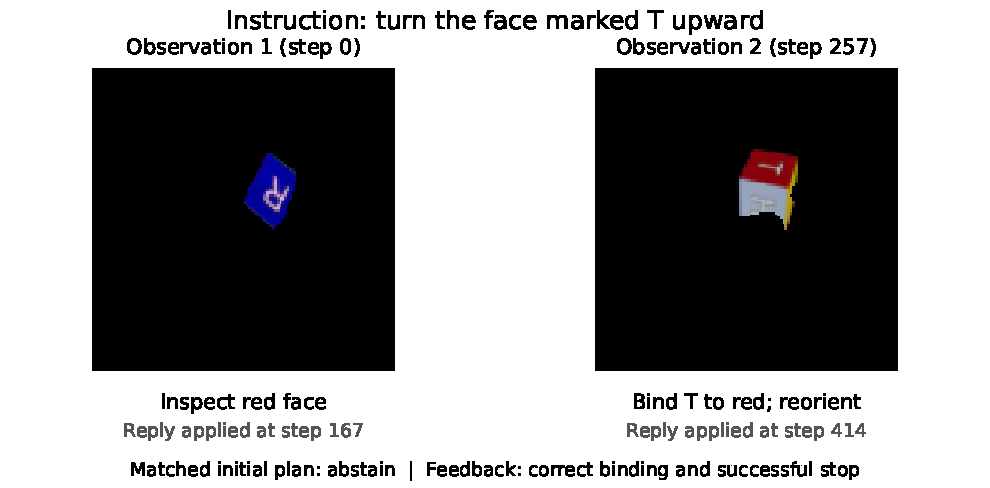
\includegraphics[width=.92\textwidth]{figures/feedback_example.pdf}
\caption{\textbf{Inspection followed by grounded execution.} Exact native model-input frames from a completed trial, enlarged without retouching. The requested letter is T. The first observation contains a visible R, and the second exposes T on the red face. Captions summarize recorded public actions. Control continues between request and reply at both observations. The two calls take 5.55 and 5.22 seconds. These are simulator images, not hardware observations.}
\label{fig:feedback-example}
\end{figure*}

\section{Q2: Control During Agent Reasoning}
\subsection{Three-seed controller evaluation}
\label{sec:collaborator-waiting}
The controller ablation uses seeds 187102, 187103 and 187104, with 40 trials per seed and method. Seed 187102 provides the first 40 trials; the other two seeds contribute a reported aggregate of 80. The main paper reports all 120 outcomes per method. Table~\ref{tab:collaborator-waiting} preserves the supplied breakdown without inferring separate counts for the latter two seeds. For learned slowing alone, we disable joint correction and keep the same initialization, data, sampling, optimizer and 2,400 updates.

\begin{table}[h]
\centering\small
\setlength{\tabcolsep}{3pt}
\begin{tabular}{lrr}
\toprule
Waiting policy & 187102 & 187103 + 187104\\
\midrule
Continue & 25 / 7 / 5 / 3 & 48 / 17 / 9 / 6\\
Fixed slowing & 30 / 4 / 0 / 6 & 58 / 9 / 8 / 5\\
Learned slowing & 28 / 1 / 7 / 4 & 54 / 6 / 7 / 13\\
Slowing + correction & 34 / 4 / 1 / 1 & 70 / 1 / 3 / 6\\
\bottomrule
\end{tabular}
\caption{Outcome breakdown for the three-seed controller study. The two columns contain 40 and 80 trials per method, respectively. Each cell lists success / waiting drop / execution drop / other failure. Other failures are not further subdivided.}
\label{tab:collaborator-waiting}
\end{table}

Q1's mapping study and Q3's image intervention use different trials. Their absolute rates need not match Q2, whose controller gains are measured within its own trial set. The initial-plan comparison shares the 40 full-feedback trials from seed 187102, as noted above.

\subsection{Waiting-controller fitting}
The waiting refit uses training collection seed 185301, validation seed 185302, and fitting seed 185311. These are training/validation seeds, not Q2 evaluation seeds. The inherited actor is updated 2,400 times. Actor batches allocate one half to pending states and one quarter each to unbound and bound execution states. Pending samples are uniform. Only the waiting outputs replace the deployed actor; execution remains unchanged. Formal Q2 evaluation uses the three seeds in Sec.~\ref{sec:collaborator-waiting}.

\subsection{Why speed and joint correction are distinct}
A scalar coefficient scales the commanded joint displacement toward the student proposal. It cannot independently change the command direction. Actual motion also depends on the joint servo and contact dynamics. To quantify that restriction, we use 17,755 pending states from 61 validation trajectory groups collected with seed 185302. These states are correlated and contain no formal evaluation trials. For normalized current position $q$, student proposal $u$, and the teacher holding action $a^*$, the best scalar action in hindsight is
\begin{equation}
 \alpha^*=\clip\!\left(\frac{(a^*-q)^\top(u-q)}{\|u-q\|_2^2},0,1\right).
\end{equation}
If $u=q$, the interpolation action is $q$ for every coefficient. The resulting error is a lower bound for any scalar-speed predictor on that state. It uses privileged teacher labels for analysis and is not a deployable policy.

\begin{table}[h]
\centering\small
\begin{tabular}{lr}
\toprule
Command design & Teacher-action MSE\\
\midrule
Continue student & 0.5953\\
Fixed slowdown & 0.6095\\
Learned slowdown & 0.4906\\
Learned slowdown + correction & 0.3870\\
\midrule
Best scalar in hindsight (bound) & 0.4330\\
\bottomrule
\end{tabular}
\caption{Held-out waiting-action fit in normalized joint-command coordinates. Lower is better. The privileged bound is distinct from the four deployable conditions. These values are not task success rates.}
\label{tab:action_space}
\end{table}
The full actor is below the scalar bound in 64.8\% of these states and has a lower mean error than the bound. This supports the additional action space provided by joint correction. It does not show that every residual is useful or that lower action error necessarily improves closed-loop success. The three-seed Q2 evaluation tests that separate question.





\subsection{Timing verification}
The request logs verify that pending requests preserve continuous logical control and that replies are applied only after their measured latency and actual completion. Replies arriving after episode termination are not applied. These checks verify the simulated delay protocol rather than wall-clock real-time operation. Q2 aggregate outcomes do not provide per-trial timing for the two additional seeds, so no timing result is extrapolated to all 120 trials.

\section{Q1: Six-Object Mapping Results}
The complete numerical table accompanies the main-paper bar chart. Each cell schedules 40 trials; service-eligible denominators are shared across methods within each condition. Object-specific weights remain fixed when the semantic mapping changes.

\begin{table*}[t]
\centering\scriptsize
\setlength{\tabcolsep}{3pt}
\begin{tabular}{llrrrrrr}
\toprule
Object & Perception & \multicolumn{3}{c}{Original mapping} & \multicolumn{3}{c}{Changed mapping}\\
\cmidrule(lr){3-5}\cmidrule(lr){6-8}
& & Rule & Fine-tuned & Full Astra & Rule & Fine-tuned & Full Astra\\
\midrule
Cube & RGB pose & 23/40 (57.5) & 30/40 (75.0) & 32/40 (80.0) & 23/40 (57.5) & 16/40 (40.0) & 32/40 (80.0)\\
Die & Noisy pose & 13/40 (32.5) & 23/40 (57.5) & 28/40 (70.0) & 1/40 (2.5) & 0/40 (0.0) & 26/40 (65.0)\\
Duck & Noisy pose & 15/38 (39.5) & 14/38 (36.8) & 25/38 (65.8) & 9/40 (22.5) & 2/40 (5.0) & 24/40 (60.0)\\
Hedgehog & Noisy pose & 17/39 (43.6) & 13/39 (33.3) & 28/39 (71.8) & 10/40 (25.0) & 2/40 (5.0) & 32/40 (80.0)\\
Pig & Noisy pose & 21/40 (52.5) & 16/40 (40.0) & 37/40 (92.5) & 15/40 (37.5) & 3/40 (7.5) & 33/40 (82.5)\\
Milk carton & Noisy pose & 13/40 (32.5) & 9/40 (22.5) & 17/40 (42.5) & 3/40 (7.5) & 1/40 (2.5) & 11/40 (27.5)\\
\bottomrule
\end{tabular}
\caption{\textbf{Q1: system comparison across six objects and two semantic mappings.} Entries give successes / common service-eligible trials (percent), retaining 40 raw trials per cell. Fine-tuned and rule baselines omit the added control modules. Each object uses its own frozen student and adaptation. The cube uses reconstructed upper-level images and RGB pose, the die rotates its visual mesh, and the four new objects permute surface letters in native RGB with noisy simulator pose. Within each object, both mappings share physical assets and weights. These mapping cohorts are separate from the native-image release comparisons. No cross-release pooled average or zero-shot object-transfer claim is made.}
\label{tab:q1-all-objects}
\end{table*}


\section{Q1: Cube System Comparisons}
\label{sec:followup}
These comparisons have their own frozen releases and trial sets. They are not additional Q2 controller seeds. Service-eligible comparisons remove the same affected slots from all arms; raw records remain archived.

\subsection{Visual-semantic interventions}
Only the agent's image changes; the pose predictor continues to receive the original image, with lighting fixed. The permuted condition assigns the next symbol in $(T,E,R,L,S,H)$ to each color face and changes the requested symbol accordingly, preserving the physical target. The masked condition hides the lettering. Image construction preserves the object's geometry, and transmitted-image hashes are verified. Seeds 183441 and 183442 provide 20 trials each, with matching physical initial states across conditions.

\begin{table}[h]
\centering\small
\setlength{\tabcolsep}{3pt}
\begin{tabular}{lrrr}
\toprule
Method & Identity & Permuted & Masked\\
\midrule
\CompletedVisualRows
\bottomrule
\end{tabular}
\caption{Completed upper-image interventions. Identity and permutation each use 40 trials. AIMI masking has one service exclusion. For its paired masking contrast the identity numerator becomes 31/39. All conditions use reconstructed face images, not the untouched native-image comparison.}
\end{table}

Fine-tuned success falls by 35 percentage points after remapping and to 7.5\% after masking. Rule-based success is 57.5\% under both identity and remapping, then zero after masking. AIMI achieves 32/40 successes under both identity and permutation, with zero of 39 eligible masked trials. Equal aggregate rates can contain different trial outcomes. The result supports performance under this tested permutation, while the binding analysis below examines reliance on prior associations.

\paragraph{Applied semantic bindings.}
We audit every applied, accepted call from the same 240 trials. The episode-file hashes match the archived results, and the last accepted skill agrees with the recorded terminal binding. Table~\ref{tab:visual-bindings} separates acquiring the correct target from completing it. Under permutation, the fine-tuned model first binds correctly in 25 trials and incorrectly in eleven, compared with 34 and four under identity. Nine of its eleven wrong-binding trials select the original color for the newly requested symbol. The rule model has six wrong-binding trials under each layout, with three following the old association after permutation. This pattern is consistent with reliance on training associations, but does not identify the model's internal mechanism.

\begin{table}[h]
\centering\small
\setlength{\tabcolsep}{3pt}
\begin{tabular}{llrrrr}
\toprule
Model & Layout & Correct & Wrong & None & Old\\
\midrule
\FollowupVisualBindingRows
\bottomrule
\end{tabular}
\caption{First accepted binding in each of 40 trials. Old counts trials with an accepted skill matching the original symbol--color association, defined only for permutation. These are the same trials as the success table, not new evaluations.}
\label{tab:visual-bindings}
\end{table}

No wrong-to-correct binding transition occurs in these bare-VLM cohorts. This is descriptive: trajectories, visibility, and opportunities for additional calls differ. Of fourteen fine-tuned false stops under permutation, ten end with a wrong binding and four with the correct binding but an independently incorrect final pose. Masking leads to no accepted binding in 36 fine-tuned trials and all forty rule-model trials. The three masked fine-tuned successes cannot establish letter grounding when that information is removed.

Identity versus permutation yields eighteen exclusive successes and four exclusive failures for the fine-tuned model (exact paired $p=0.00434$), versus ten and ten for the rule model ($p=1.0$). The final analysis applies Holm correction across six planned image contrasts, giving adjusted $p=0.0130$ for the fine-tuned mapping contrast. The single deterministic remapping and reconstructed upper images limit generalization claims. AIMI has five exclusive identity successes and five exclusive permutation successes ($p=1.0$).


\subsection{Native-image comparison and failure audit}
Seeds 185451 and 185452 give 40 matched trials per method with no service exclusions. The AIMI system gives 35 successes, three execution-phase drops, one wrong-binding false stop, and one abstention. The bare fine-tuned system gives 30 successes, nine execution drops, and one horizon failure. The bare rule system gives 17 successes, twelve drops, ten false stops, and one horizon failure. Its drops include two during startup waiting. AIMI makes 101 calls, fine-tuning 117, and the rule baseline 126. Median latencies are 4.349, 0.099 and 1.104 seconds.

The three AIMI drops occur during inspection before final target binding. One is 59 control steps after the most recent applied inspection command, and the others are 36 and 24 steps after it. These intervals describe timing, not causal attribution. The false-stop episode binds R to cyan rather than blue. Its measured error to the declared target is 0.057 radians, while true requested-target error is 3.079 radians. It is a semantic binding failure and cannot simply be assigned to pose estimation. The abstention follows four inspections without a declared target. A favorable instantaneous pose during that trajectory does not meet the autonomous success rule.

\section{Q1: Native-Layout Dice Extension}
\label{sec:dice-extension}
The die is a wooden object with one through six native textured pips, rendered at $512\times512$ with the hand. Three methods each run 40 matched trials over seeds 186301 and 186302. The independent audit verifies all 120 records, canonical targets, paired reset states, response latency and baseline isolation. No trial is service-excluded.

\paragraph{Object-specific motor interface.}
The released feedforward actor uses ten frames of normalized input. Its goal-related channels are replaced by a learned reconstruction of eight conditioning features. For each frame, a 768-dimensional latent is normalized and encoded to 32 dimensions. The adapter combines it with the four measured quaternion components and their outer product, then applies layers of widths 256, 128, and 8. The original actor and observation normalization remain frozen. Inference receives physical history of shape $10\times116$ and continuous latent history of shape $10\times768$. It receives no true target quaternion, target index or table-based reconstruction of its conditioning features.

\paragraph{Perception, control and stop policy.}
The die uses the released simulator-pose noise, bias, failure, jitter and delay model. There is no image pose estimator in these trials. All upper methods receive the same RGB and image-only crop. The physical horizon is 120 seconds at 20~Hz and the stop gate is checked at 3~Hz. A reply cannot be applied before $\lceil20L\rceil$ steps, while control continues. The drop boundary and independent full-quaternion success tolerance remain 0.24 metres and 0.16 radians.

AIMI uses one object-specific maintenance actor during pending and ordinary execution. Its calibrated completion model learns a bounded correction to measured angular error and an uncertainty term. It accepts when the calibrated upper bound is at most 0.16 radians. Once a correct count is declared and the state is not inspection, this gate may stop even with a further request pending. The bare baselines use no learned maintenance or completion module and stop on the measured-angle criterion only when no request is pending. Thus these are complete-system comparisons, not isolated tests of the semantic models or a replication of the cube's shared measured gate.

\begin{table}[t]
\centering\small
\begin{tabular}{lrrrr}
\toprule
System & Success & \% & Drops & Calls\\
\midrule
AIMI & 24/40 & 60.0 & 15 & 63\\
Fine-tuned VLM, bare & 20/40 & 50.0 & 8 & 141\\
Rule VLM, bare & 17/40 & 42.5 & 7 & 154\\
\bottomrule
\end{tabular}
\caption{Completed native-layout die comparison. No service exclusions. The independent success definition is shared; internal control and stop modules differ by system.}
\end{table}

AIMI's 95\% Wilson interval is [44.6, 73.7]\%, versus [35.2, 64.8]\% for fine-tuning and [28.5, 57.8]\% for rules. AIMI has ten exclusive successes against six for fine-tuning (exact paired $p=0.4545$), and eleven against four for rules ($p=0.1185$). These exploratory comparisons do not establish superiority. AIMI has twelve startup drops, three execution drops and one false stop. Fine-tuning has eight execution drops, seven false stops and five horizon failures. Rules have seven startup drops, six false stops and ten horizon failures. Median request latencies are 5.63, 0.124 and 1.16 seconds, respectively.

\section{Q1: Dice Visual-Layout Transfer}
\label{sec:dice-layout}
\begin{figure*}[t]
\centering
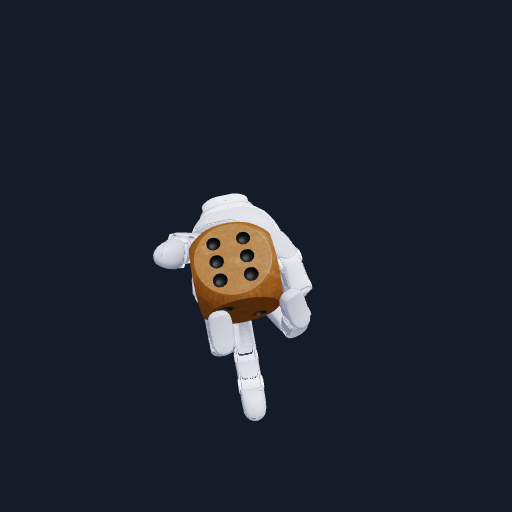
\includegraphics[width=.38\textwidth]{data/dice_visual_layout_20261102/qualitative_request_02.png}\hspace{.04\textwidth}
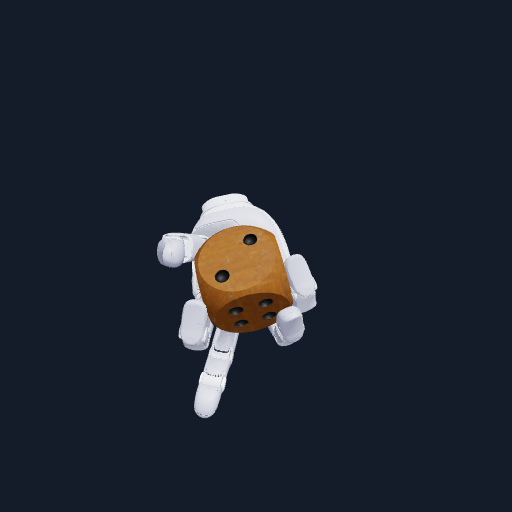
\includegraphics[width=.38\textwidth]{data/dice_visual_layout_20261102/qualitative_request_03.png}
\caption{A recorded permuted-layout episode requesting two dots upward. Left: probing physical skill 3 exposes six dots. Right: probing skill 1 exposes two dots. AIMI then binds the target to skill 1 and stops with an independently measured orientation error of 0.025 radians. Images are the actual model inputs. This first scheduled trial was selected after its outcome and illustrates one successful sequence, not a reliability estimate.}
\label{fig:dice-probe}
\end{figure*}

The six cells use identity or a 120-degree visual-mesh rotation about a body diagonal, crossed with three methods. Each cell contains 40 scheduled trials over seeds 186701 and 186702, with matched physical targets and initial states. Collision, inertia and formal solver settings are unchanged. The mesh has slight asymmetries, so this is a visual-layout intervention rather than a pure texture edit. Independent deterministic diagnostics produce identical 32-step state/action traces for native, identity and permuted layers. The formal solver retains its original settings.

\paragraph{Input and motor contract.}
Printed counts are separated from fixed physical motor IDs. Skills 1--6 display counts $[1,2,3,4,5,6]$ in identity and $[2,4,6,1,3,5]$ after rotation. This table is used only to construct task instructions and score outcomes. Models receive no layout table, and their commands are not inversely remapped. The learned VLM's continuous 768-dimensional output is applied unchanged. Both layouts share an explicit skill-ID prompt that differs from the native-main prompt, making identity a control for that common change. The VLM retains its native-layout-trained weights. This measures zero-shot layout transfer, not performance after training on permuted examples.

AIMI receives updated RGB, action/observation history and noisy feedback and can probe skills. The bare VLMs receive only current RGB and instruction, with their original fallback inspection schedule. From a single view, a new printed-count-to-motor-ID association may be ambiguous without a stable face reference. The comparison therefore measures complete systems, not a controlled effect of model scale or fine-tuning alone. Dice maintenance and stopping modules remain as documented above. The shared primary success predicate is unchanged.

\begin{table}[t]
\centering\small
\begin{tabular}{lrr}
\toprule
System & Identity & Permuted\\
\midrule
\DiceLayoutRows
\bottomrule
\end{tabular}
\caption{Dice visual-layout transfer. All 240 scheduled trials are service-eligible. Forty reset states and physical goals are matched across all six cells.}
\label{tab:dice-layout}
\end{table}

\paragraph{Results and paired uncertainty.}
AIMI completes 28/40 identity trials and 26/40 permuted trials. Their 95\% Wilson intervals are [54.6, 81.9]\% and [49.5, 77.9]\%. Fine-tuning changes from 23/40 to 0/40, and rules from 13/40 to 1/40. Four paired states succeed only for identity AIMI and two only for permuted AIMI. The absence of a detected difference does not establish equivalence or robustness to other layouts. Table~\ref{tab:dice-layout-tests} reports all seven exploratory paired contrasts without multiple-testing adjustment. The native-main results are a separate cohort and must not be pooled with this study.

\begin{table}[t]
\centering\small
\setlength{\tabcolsep}{3pt}
\begin{tabularx}{\linewidth}{@{}Xrrr@{}}
\toprule
Contrast A versus B & A only & B only & Exact $p$\\
\midrule
\DiceLayoutTestRows
\bottomrule
\end{tabularx}
\caption{Exploratory exact two-sided McNemar tests on 40 paired states. Tests are unadjusted. I and P denote identity and permuted layouts.}
\label{tab:dice-layout-tests}
\end{table}

\paragraph{Binding and control failures.}
Permuted AIMI has 27 trials with a correct binding to a skill ID different from the printed count, and 26 complete successfully. It applies inspection in 32 trials and first binds after inspection in 27. No wrong-to-correct binding transition is observed. Its failures comprise seven startup drops, one execution drop, five abstentions and one wrong-binding stop. These traces describe evidence gathering before commitment, not recovery from an already executed incorrect binding.

The permuted fine-tuned VLM has 31 wrong-binding stops, five horizons and four execution drops. All 31 wrong-binding stops report the native same-number skill. Code review confirms that RGB and instruction enter the backbone and learned latent head, with no service-side assignment from requested count to skill. In identity, it binds correctly in 36 trials but succeeds in 23, illustrating a separate control/stop limitation. The permuted rule model has 32 wrong-binding stops, four horizons, three drops and one success; 24 of its wrong-binding stops select the native same-number skill. These post-hoc diagnostics are consistent with reliance on native associations. They do not establish memorization as an exclusive cause, especially given the baseline's limited observation history.



\paragraph{Audit and scope.}
The independent audit checks all 240 trials, 69 frozen source files, matched resets, model-request image hashes, delayed response application, continuous VLM latents and canonical-quaternion scoring. A separate SciPy calculation verifies all six Wilson intervals and seven exact paired tests. No service exclusions, outcome replacements or post-test model changes occur. Trace diagnostics were developed while cells were completing and are explicitly post-hoc. Earlier invalid digit-overlay attempts are excluded and preserved separately. One changed layout, one native-trained local model and object-specific motor weights do not establish broad semantic or geometric generalization.

\section{Q1: Four Additional Objects}
Duck, hedgehog, pig and milk carton each contribute six cells of forty raw trials, totaling 960. Each object uses its own frozen student and adaptation, native marked RGB for semantic decisions, and noisy simulator pose for motor control. Bare VLM baselines omit the added control modules. We preserve every recorded outcome. Two historical duck service failures and one hedgehog service failure affect only original-mapping cells. Common service-eligible panels remove the corresponding slots from all three methods. All changed-mapping cells retain forty trials.

The full audit covers all 960 episodes, 320 within-mapping initial-image groups and 160 physical-state groups. Seventeen image comparisons differ in one color channel of one pixel by one 8-bit level. Saved model-request pixels and delivered-input hashes match strictly. One duck original-mapping AIMI reset (slot 7) differs from the other conditions in one quaternion component by $2.98\times10^{-8}$. The normalized angular difference is $5.77\times10^{-8}$ radians, with identical initial image pixels. We retain this explicitly reviewed numerical exception rather than claiming bitwise reset equality. All other recorded state components match exactly.

As a sensitivity analysis, removing slot 7 from every method gives original-mapping successes of 24/37 for AIMI, 13/37 for fine-tuning and 15/37 for rules. Removing it from the changed mapping gives 23/39, 2/39 and 9/39. The ordering is unchanged. The main table retains the frozen service-exclusion rule. This post-run sensitivity check does not replace outcomes or change the success definition.

\section{Q1: Language and Wording Coverage Across Three Objects}
\label{sec:language-supp}
Three separate cohorts contribute 2,160 recorded trials: cube, duck and hedgehog, each with three systems, two languages, two wording templates per language and 60 trials per cell. Cube seeds are 210501--210503, duck seeds 210601--210603, and hedgehog seeds 210701--210703, twenty trials per seed. Each of six goals occurs ten times per cell. These are evaluation blocks, not independent training seeds. Within each object, the same 60 reset seeds and physical goals are reused across methods and instruction variants. Four prompt variants must not be pooled as 240 independent physical tasks.

\paragraph{Intervention and deployment.}
Mapping, task criterion and object-specific weights remain fixed within each system. Cube retains its visual pose estimator, goal bank, latent student, 30-Hz control and measured-pose stopping; AIMI uses its paper-selected waiting and execution actors. Duck and hedgehog use their own latent students, 20-Hz control and noisy simulator-pose feedback; AIMI additionally uses object-specific learned maintenance and completion correction. Bare local baselines omit these added actors. All systems use the independently scored 0.16-radian tolerance. Upper RGB is 120-by-120 for cube and 512-by-512 for duck and hedgehog. The English-trained fine-tuned models receive the requested instructions without Chinese retraining. The rule baseline additionally uses localized task/output instructions for Chinese conditions. This is deployed-system language coverage, not an isolated change to the user sentence for every backend, a shared-policy transfer test, or a causal test of fine-tuning. Exact prompts are retained in the evidence bundle.

\paragraph{Service eligibility and raw records.}
The main-paper language table reports completion conditional on service availability. Within each object and instruction condition, the union of infrastructure-affected slots is removed from all three methods, including any successful baseline outcome at that slot. Thus each row comparison uses identical physical tasks and the same denominator. These rates do not measure end-to-end service reliability. This reporting choice was made after inspecting the raw outcomes; it is not described as preregistered. Table~\ref{tab:language-raw} retains every scheduled slot and Table~\ref{tab:language-exclusions} lists exclusions. No excluded slot is replaced; continuations visit only unvisited slots. Physical drops, incorrect stopping, abstention and task-horizon failures remain in the denominator. Infrastructure faults include TLS/proxy failures and server overload, not model grounding or control errors.

\begin{table}[t]
\centering\footnotesize
\setlength{\tabcolsep}{2pt}
\begin{tabular}{@{}lrrrr@{}}
\toprule
 & \multicolumn{2}{c}{English} & \multicolumn{2}{c}{Chinese}\\
System & Standard & Rewrite & Standard & Rewrite\\
\midrule
\multicolumn{5}{l}{\textit{Cube: $n=60, 60, 60, 60$}}\\
AIMI & 42/60 & 47/60 & 48/60 & 36/60\\
Fine-tuned VLM & 42/60 & 44/60 & 46/60 & 47/60\\
Rule VLM & 28/60 & 27/60 & 18/60 & 19/60\\
\midrule
\multicolumn{5}{l}{\textit{Duck: $n=60, 60, 60, 60$}}\\
AIMI & 41/60 & 40/60 & 41/60 & 46/60\\
Fine-tuned VLM & 23/60 & 18/60 & 19/60 & 21/60\\
Rule VLM & 30/60 & 15/60 & 20/60 & 19/60\\
\midrule
\multicolumn{5}{l}{\textit{Hedgehog: $n=60, 60, 60, 60$}}\\
AIMI & 44/60 & 46/60 & 39/60 & 46/60\\
Fine-tuned VLM & 23/60 & 19/60 & 21/60 & 15/60\\
Rule VLM & 28/60 & 23/60 & 21/60 & 22/60\\
\bottomrule
\end{tabular}
\caption{Raw completion counts over all scheduled trials, retaining infrastructure failures in the denominator. These are separate object-specific cohorts; the four instruction variants reuse physical tasks.}
\label{tab:language-raw}
\end{table}

\begin{table}[t]
\centering\footnotesize
\setlength{\tabcolsep}{2pt}
\begin{tabular}{@{}lrrrr@{}}
\toprule
 & \multicolumn{2}{c}{English} & \multicolumn{2}{c}{Chinese}\\
System & Standard & Rewrite & Standard & Rewrite\\
\midrule
\multicolumn{5}{l}{\textit{Cube}}\\
AIMI & 4 & 1 & 3 & 7\\
Fine-tuned VLM & 0 & 0 & 0 & 0\\
Rule VLM & 0 & 0 & 0 & 0\\
\midrule
\multicolumn{5}{l}{\textit{Duck}}\\
AIMI & 0 & 1 & 0 & 0\\
Fine-tuned VLM & 0 & 0 & 0 & 0\\
Rule VLM & 0 & 0 & 0 & 0\\
\midrule
\multicolumn{5}{l}{\textit{Hedgehog}}\\
AIMI & 0 & 0 & 8 & 0\\
Fine-tuned VLM & 0 & 0 & 0 & 0\\
Rule VLM & 0 & 0 & 0 & 0\\
\bottomrule
\end{tabular}
\caption{Service-excluded trial counts, each out of 60 scheduled slots. All raw records are retained.}
\label{tab:language-exclusions}
\end{table}


\paragraph{Continuation and availability.}
Service failures interrupted the hedgehog queue. Only unvisited tasks resumed, using separate workers and verified direct HTTPS to the same endpoint after a further SSL failure. Model, weights, prompts, seeds, scoring and one-attempt transport policy remained fixed. All prior outcomes, errors, actual latencies and scheduler changes are retained in the archive.

\paragraph{State pairing and image sensitivity.}
Cube and duck initial-state hashes match exactly across methods and instruction conditions. Four hedgehog slots differ only in object-quaternion components by at most $5.96\times10^{-8}$; all other recorded state components match exactly. A post-run numerical reset audit uses a $10^{-6}$ component tolerance, and the strict sensitivity below removes any nonidentical hashes. Cube first-image hashes match exactly. Some duck and hedgehog renders differ at the pixel level; these do not alter the service-eligible main denominator. Table~\ref{tab:language-sensitivity} additionally requires identical initial-state and first-image hashes across all three methods in a condition. All strict paired tests are retained in the data export. The duck differences involve six slots, at most two RGB pixels and one channel level per pixel in 512-by-512 images. Hedgehog image differences involve 12 slots, at most two RGB pixels and one channel level in the same resolution.

\begin{table}[t]
\centering\footnotesize
\setlength{\tabcolsep}{2pt}
\begin{tabular}{@{}lrrrr@{}}
\toprule
 & \multicolumn{2}{c}{English} & \multicolumn{2}{c}{Chinese}\\
System & Standard & Rewrite & Standard & Rewrite\\
\midrule
\multicolumn{5}{l}{\textit{Cube: $n=56, 59, 57, 53$}}\\
AIMI & 42/56 & 47/59 & 48/57 & 36/53\\
Fine-tuned VLM & 40/56 & 43/59 & 43/57 & 43/53\\
Rule VLM & 27/56 & 27/59 & 18/57 & 17/53\\
\midrule
\multicolumn{5}{l}{\textit{Duck: $n=56, 57, 57, 56$}}\\
AIMI & 39/56 & 40/57 & 40/57 & 43/56\\
Fine-tuned VLM & 21/56 & 17/57 & 18/57 & 19/56\\
Rule VLM & 29/56 & 15/57 & 20/57 & 19/56\\
\midrule
\multicolumn{5}{l}{\textit{Hedgehog: $n=52, 52, 46, 55$}}\\
AIMI & 38/52 & 40/52 & 36/46 & 43/55\\
Fine-tuned VLM & 19/52 & 15/52 & 17/46 & 13/55\\
Rule VLM & 22/52 & 18/52 & 16/46 & 19/55\\
\bottomrule
\end{tabular}
\caption{Strict pairing sensitivity: common service-eligible slots additionally require identical initial-state and first-image hashes across all three methods. Numerators are successes. This is separate from the main service-eligible estimand.}
\label{tab:language-sensitivity}
\end{table}


\paragraph{Paired inference.}
Two-sided exact McNemar tests use discordant pairs. Method tests use the same common three-method service-eligible panels as the main table. A language/wording contrast excludes the union of service-affected slots in its two arms; its denominator can differ from a main-table denominator. Holm correction is applied jointly across three objects: one family of 36 language/wording contrasts and a separate family of 36 method contrasts. The strict state-and-image-matched sensitivity applies the same corrections separately. Tables~\ref{tab:language-wording-tests} and~\ref{tab:language-method-tests} report all main adjusted tests. No language/wording contrast survives Holm correction. 20 of 36 method contrasts survive correction. Strict state-and-image-matched sensitivity changes the 0.05 significance decision in 0 of the 72 contrasts; all discordant counts and adjusted values are archived. These tests do not isolate model-only or controller-only effects.

\begin{table}[t]
\centering\footnotesize
\setlength{\tabcolsep}{2pt}
\begin{tabular}{@{}lrrrr@{}}
\toprule
 & \multicolumn{2}{c}{EN vs. ZH} & \multicolumn{2}{c}{Standard vs. rewrite}\\
System & Standard & Rewrite & English & Chinese\\
\midrule
\multicolumn{5}{l}{\textit{Cube}}\\
AIMI & 1.0000 & 1.0000 & 1.0000 & 0.7637\\
Fine-tuned VLM & 1.0000 & 1.0000 & 1.0000 & 1.0000\\
Rule VLM & 0.4529 & 1.0000 & 1.0000 & 1.0000\\
\midrule
\multicolumn{5}{l}{\textit{Duck}}\\
AIMI & 1.0000 & 1.0000 & 1.0000 & 1.0000\\
Fine-tuned VLM & 1.0000 & 1.0000 & 1.0000 & 1.0000\\
Rule VLM & 1.0000 & 1.0000 & 0.0936 & 1.0000\\
\midrule
\multicolumn{5}{l}{\textit{Hedgehog}}\\
AIMI & 1.0000 & 1.0000 & 1.0000 & 1.0000\\
Fine-tuned VLM & 1.0000 & 1.0000 & 1.0000 & 1.0000\\
Rule VLM & 1.0000 & 1.0000 & 1.0000 & 1.0000\\
\bottomrule
\end{tabular}
\caption{Exact paired language/wording tests, Holm-adjusted jointly over 36 contrasts across three objects. Non-significance does not establish equivalence.}
\label{tab:language-wording-tests}
\end{table}
\begin{table}[t]
\centering\footnotesize
\setlength{\tabcolsep}{5pt}
\begin{tabular}{@{}lrrr@{}}
\toprule
Condition & AIMI--FT & AIMI--Rule & FT--Rule\\
\midrule
\multicolumn{4}{l}{\textit{Cube}}\\
EN standard & 1.0000 & 0.1220 & 0.1487\\
EN rewrite & 1.0000 & 0.0102 & 0.0424\\
ZH standard & 1.0000 & $<0.0001$ & $<0.0001$\\
ZH rewrite & 1.0000 & 0.0017 & $<0.0001$\\
\midrule
\multicolumn{4}{l}{\textit{Duck}}\\
EN standard & 0.0258 & 0.3458 & 1.0000\\
EN rewrite & 0.0043 & 0.0011 & 1.0000\\
ZH standard & 0.0043 & 0.0102 & 1.0000\\
ZH rewrite & $<0.0001$ & 0.0001 & 1.0000\\
\midrule
\multicolumn{4}{l}{\textit{Hedgehog}}\\
EN standard & 0.0025 & 0.1120 & 1.0000\\
EN rewrite & $<0.0001$ & 0.0004 & 1.0000\\
ZH standard & 0.0013 & 0.0041 & 1.0000\\
ZH rewrite & $<0.0001$ & 0.0011 & 1.0000\\
\bottomrule
\end{tabular}
\caption{Exact paired method tests on the main common service-eligible panels, Holm-adjusted over a separate family of 36 contrasts. FT denotes fine-tuning. Strict pairing sensitivity tests are archived.}
\label{tab:language-method-tests}
\end{table}


\paragraph{Scope and evidence.}
Two languages and two templates per language, with six fixed targets and one mapping per object, do not establish broad multilingual generalization or equivalence. Earlier misconfigured runs are excluded; historical native/mapping cohorts remain separate. The sanitized archive retains all 2,160 outcomes, 72 main and 72 sensitivity comparisons, prompts, schedules and checksums.

\section{Q4: Independent Pose Estimation under Hand Occlusion}
\label{sec:pose-occlusion}
This supporting perception study for Q4 evaluates fixed RGB and RGB-D estimators on a 58.5~mm lettered cube. Its RGB model differs from the frozen agent CNN, and its pose recalls do not update agent success counts.

\paragraph{Sampling and scoring.}
Three test seeds (31001--31003), four camera pitches ($0^\circ$, $60^\circ$, $90^\circ$, $105^\circ$), and 512 frames per group yield 6,144 observations in 48 environment clusters. RGB, RGB-D, their no-hand controls and perturbed-depth RGB-D produce 30,720 predictions. Collection records four geometry rejections; 6,139 admitted observations contain the full object.

Recall requires translation error $<10$~mm and full rotation error $<10^\circ$, without cube-symmetry minimization. Invalid predictions count as failures. Secondary recall uses 5~mm and $5^\circ$. ADD uses 6,144 nominal-cube surface points and a threshold of 0.1 diameter. All evaluated thresholds are strict, and no samples lie on the primary boundaries.

\begin{table}[t]
\centering\small
\begin{tabular}{lrrr}
\toprule
Hand occlusion & Frames & RGB & RGB-D \\
\midrule
{[0,25\%)} & 2,891 & 66.17 & 97.61 \\
{[25,50\%)} & 1,964 & 19.91 & 55.45 \\
{[50,75\%)} & 1,198 & 0.17 & 5.51 \\
{[75,100\%]} & 91 & 0.00 & 0.00 \\
\midrule
All & 6,144 & 37.53 & 64.73 \\
\bottomrule
\end{tabular}

\caption{Independent pose recall (\%) under hand occlusion. All frames remain in the denominator, including invalid predictions. Occlusion is associated with viewpoint in this sampling design.}
\label{tab:pose-occlusion}
\end{table}

\paragraph{Accuracy and uncertainty.}
RGB passes on 2,306/6,144 observations and RGB-D on 3,977/6,144, a difference of 27.20 percentage points. The reported 95\% intervals are [36.60,38.48]\% for RGB, [64.02,65.46]\% for RGB-D, and [26.07,28.30] points for the paired difference. Intervals use 10,000 paired bootstrap draws of whole environment clusters, stratified by seed, retaining their views and temporal observations together. They describe sampling variation for this object and these test seeds, not variation across trained models or unseen objects. Table~\ref{tab:pose-occlusion} shows that gains concentrate in light and moderate occlusion. At 50--75\%, RGB-D recall is only 5.51\%, and both systems fail all 91 observations at $\geq75\%$.

\begin{table}[t]
\centering\small
\begin{tabular}{lrr}
\toprule
Metric & RGB & RGB-D \\
\midrule
Recall, 10 mm / 10 deg. (\%) & 37.53 & 64.73 \\
Recall, 5 mm / 5 deg. (\%) & 14.63 & 47.56 \\
ADD recall (\%) & 38.35 & 71.48 \\
Translation mean (mm)$^{*}$ & 57.56 & 6.26 \\
Rotation mean (deg.)$^{*}$ & 12.28 & 10.82 \\
Invalid predictions & 69/6144 & 1/6144 \\
\bottomrule
\end{tabular}

\caption{Secondary pose metrics. All recall denominators include invalid predictions. $^{*}$Mean errors use valid predictions only and must be interpreted with the invalid counts. Threshold comparisons are strict.}
\label{tab:pose-metrics}
\end{table}

\paragraph{Paired controls and sensitivity.}
Removing hand occlusion at matched poses gives recall of 76.90\% for RGB and 99.89\% for RGB-D. The overall occlusion-associated loss is therefore 39.37 versus 35.16 points, with a paired reduction of 4.22 points [2.77,5.62]. This reduction is not uniform: at 50--75\% occlusion, the loss is 72.20 versus 94.49 points. The higher unoccluded RGB-D ceiling does not imply robustness when most of the object is hidden. The no-hand RGB render retains soft Gaussian-splat boundaries, whereas the occluded image uses a hard visible-object mask, which also limits this control. Restricting to fully framed observations gives 37.56\% versus 64.78\%, similar to the full cohort.

Adding 1~mm Gaussian ray-depth noise and dropping 20\% of points yields RGB-D recall of 3,973/6,144 (64.66\%). This is a sensitivity check, not a calibrated physical depth-camera error model. Per-seed RGB/RGB-D recall is 37.30/64.89\%, 37.70/64.36\%, and 37.60/64.94\%. Viewpoint and occlusion covary: recall at nominal view is 76.04/99.80\%, versus 0.85/4.23\% at $105^\circ$.

\paragraph{Training and interpretation.}
The RGB system uses development-selected letterboxing and its existing PnP decoder. RGB-D uses the supplied epoch-1812 weights. Training histories and camera adaptation differ, so this is not a matched-budget architecture or depth-input ablation. RGB-D training manifests record 20,000 samples from seeds 43--50, validation uses seed 2027, and the test seeds do not overlap. Only nine training entries have more than 50\% occlusion. This post-hoc manifest observation is consistent with the severe-occlusion failure but is not causal evidence, and the full training imagery has not been re-audited. The old RGB training-data lineage is incomplete.

The evaluation uses simulator pose labels, ideal target segmentation, and virtual co-located depth. Real-camera calibration and Gaussian-splat appearance assets are part of the setup, so it should not be described as using no real-world information. The evidence supports improved simulated pose accuracy over this RGB deployment, with a clear severe-occlusion limit. It does not yet establish improved agent completion or real-camera accuracy. The earlier 39/40 original pose-goal versus 35/40 latent-student physical-reach diagnostic used the frozen agent CNN and is a separate experiment.

\paragraph{Evidence provenance.}
The supplied integrity report records 129 unchanged frozen files, shared finite ground truth, and pose-error recomputation within $2.28\times10^{-13}$~mm and $1.01\times10^{-11}$ degrees. Paper integration verifies file hashes and re-sums twelve shard counts. Bootstrap intervals and per-frame checks retain delivery provenance. Protocol/model hashes are archived; the final reproduction package still needs sanitized per-frame records.

\section{Q4: Physical-Hand Evaluation}
\label{sec:hardware}
We evaluate the complete Rule, Fine-tuned and AIMI systems on a Revo3 hand with four physical objects: cube, die, ball and duck. Each object--method combination has 20 trials, totaling 80 per method and 240 overall. RGB images provide estimated object pose to the control policy, following the ViserDex-based deployment interface. The ball belongs to this hardware cohort and is not an additional Q1 simulation object.

\begin{table}[!htbp]
\centering\small
\setlength{\tabcolsep}{3pt}
\begin{tabular}{lccc}
\toprule
Object & Rule & Fine-tuned & AIMI\\
\midrule
Cube & 9/20 (45\%) & 15/20 (75\%) & \textbf{18/20 (90\%)}\\
Die & 8/20 (40\%) & 14/20 (70\%) & \textbf{18/20 (90\%)}\\
Ball & 9/20 (45\%) & 13/20 (65\%) & \textbf{19/20 (95\%)}\\
Duck & 6/20 (30\%) & 11/20 (55\%) & \textbf{15/20 (75\%)}\\
\midrule
Total & 32/80 (40\%) & 53/80 (66.25\%) & \textbf{70/80 (87.5\%)}\\
\bottomrule
\end{tabular}
\caption{\textbf{Q4: real-hand task completion.} Successes/trials and rates for the four physical objects. Every object--method cell contains 20 trials. Success requires reaching the requested target and stopping within $15^\circ$ without dropping the object.}
\label{tab:hardware-results}
\end{table}


A trial succeeds when the robot reaches the requested target, stops with orientation error at most $15^\circ$, and does not drop the object. This hardware criterion is distinct from the simulation tolerance of 0.16 radians. Table~\ref{tab:hardware-results} reports 32/80, 53/80 and 70/80 successes for Rule, Fine-tuned and AIMI. Equal trials per object make the pooled rate equal to the object-averaged rate. These complete-system results do not isolate the effect of perception adaptation or measure an additional post-stop holding period.

\TODO{Add the camera/scoring setup and recorded physical-hand sequences.} The image layouts below reserve space for the task instruction, inspection views, target binding and final presentation.



\begin{figure*}[t]
\centering
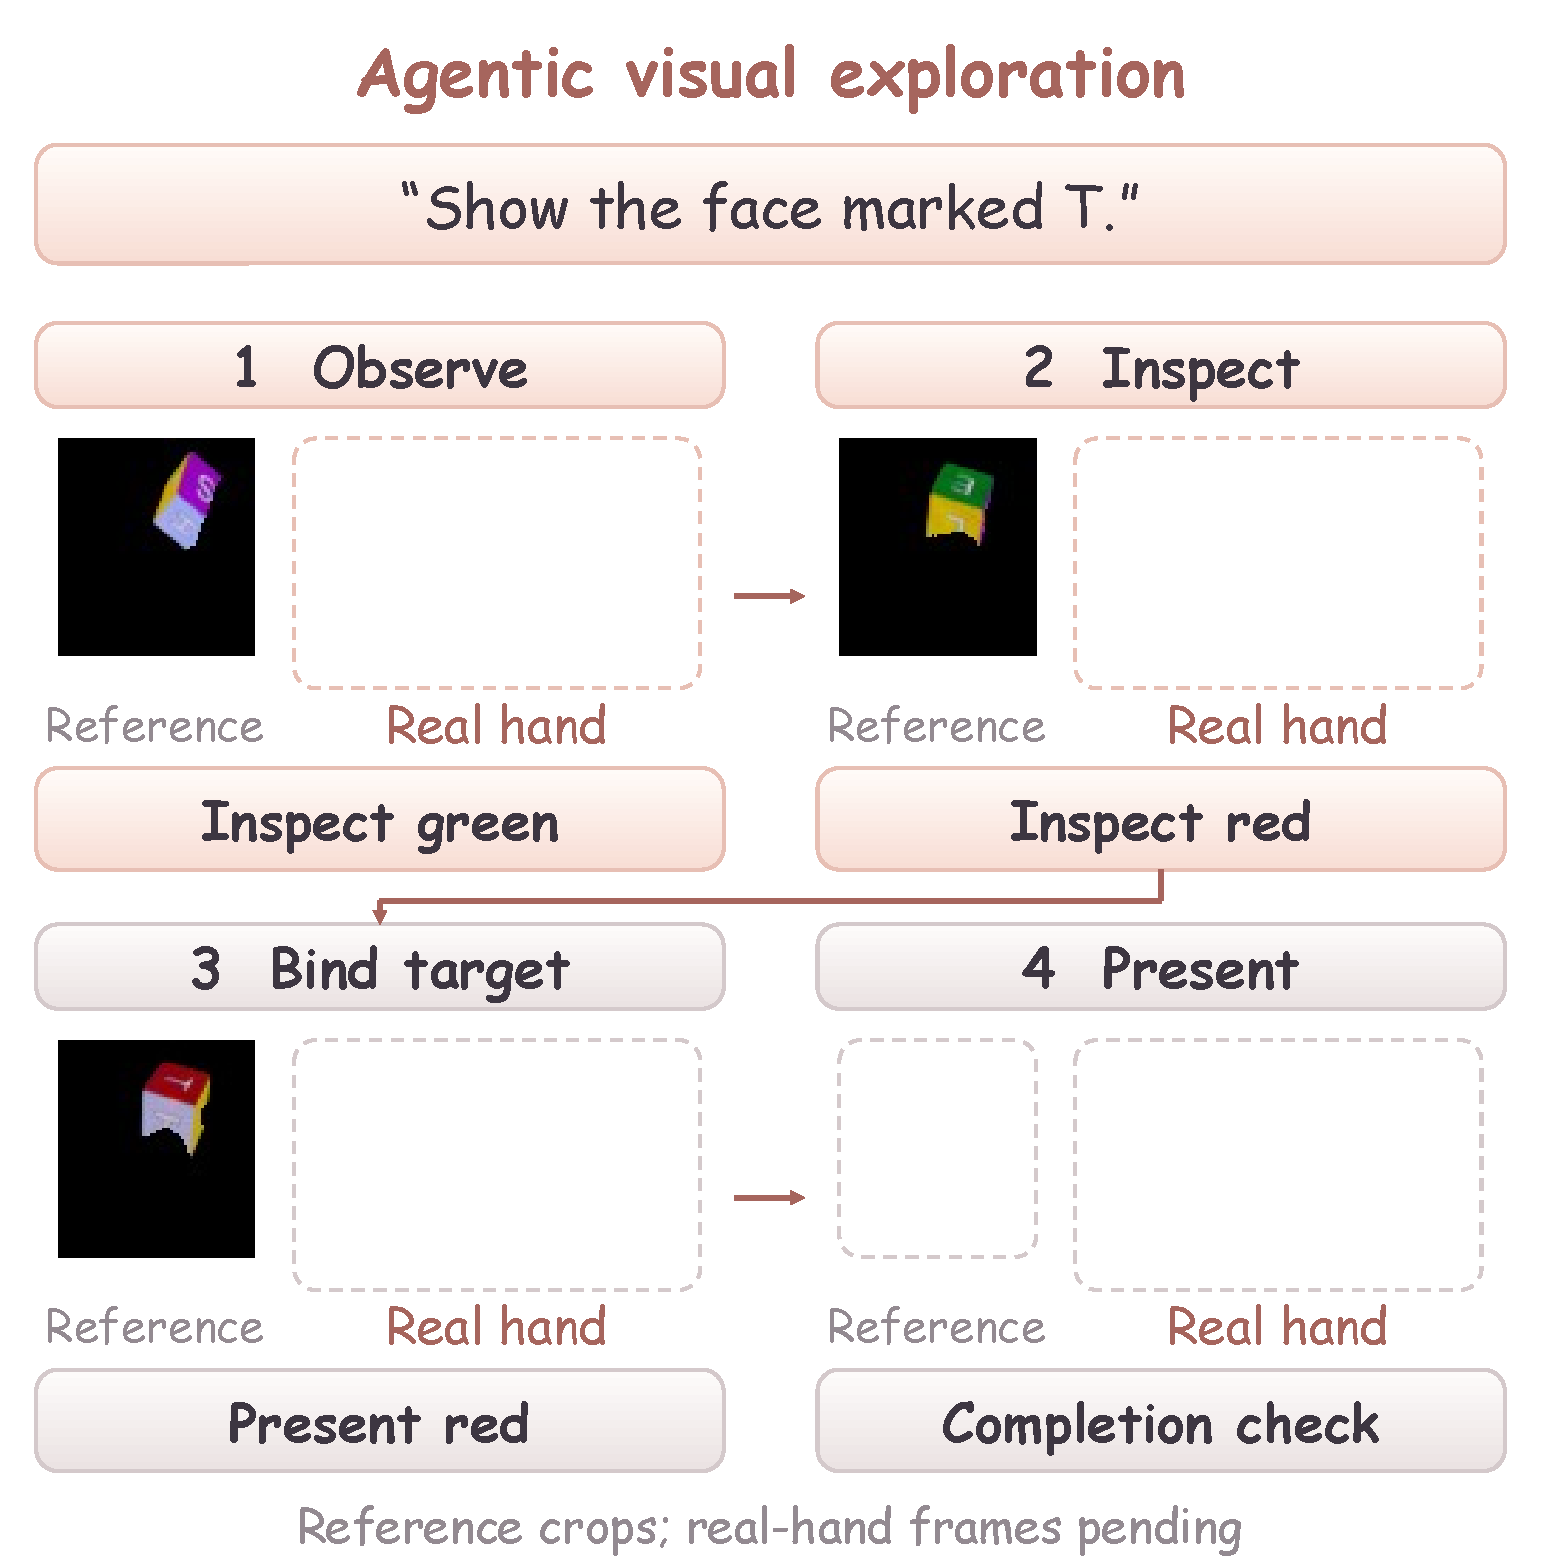
\includegraphics[width=0.50\textwidth]{figures/imported/aimi_exploration.pdf}
\caption{\textbf{Planned inspection and presentation sequence.} Reference crops illustrate observing, inspecting, binding, and presenting a requested face. Real-hand image slots remain empty. This is a protocol mockup, not a physical-robot result.}
\label{fig:sim-real-protocol}
\end{figure*}

\begin{figure*}[t]
\centering
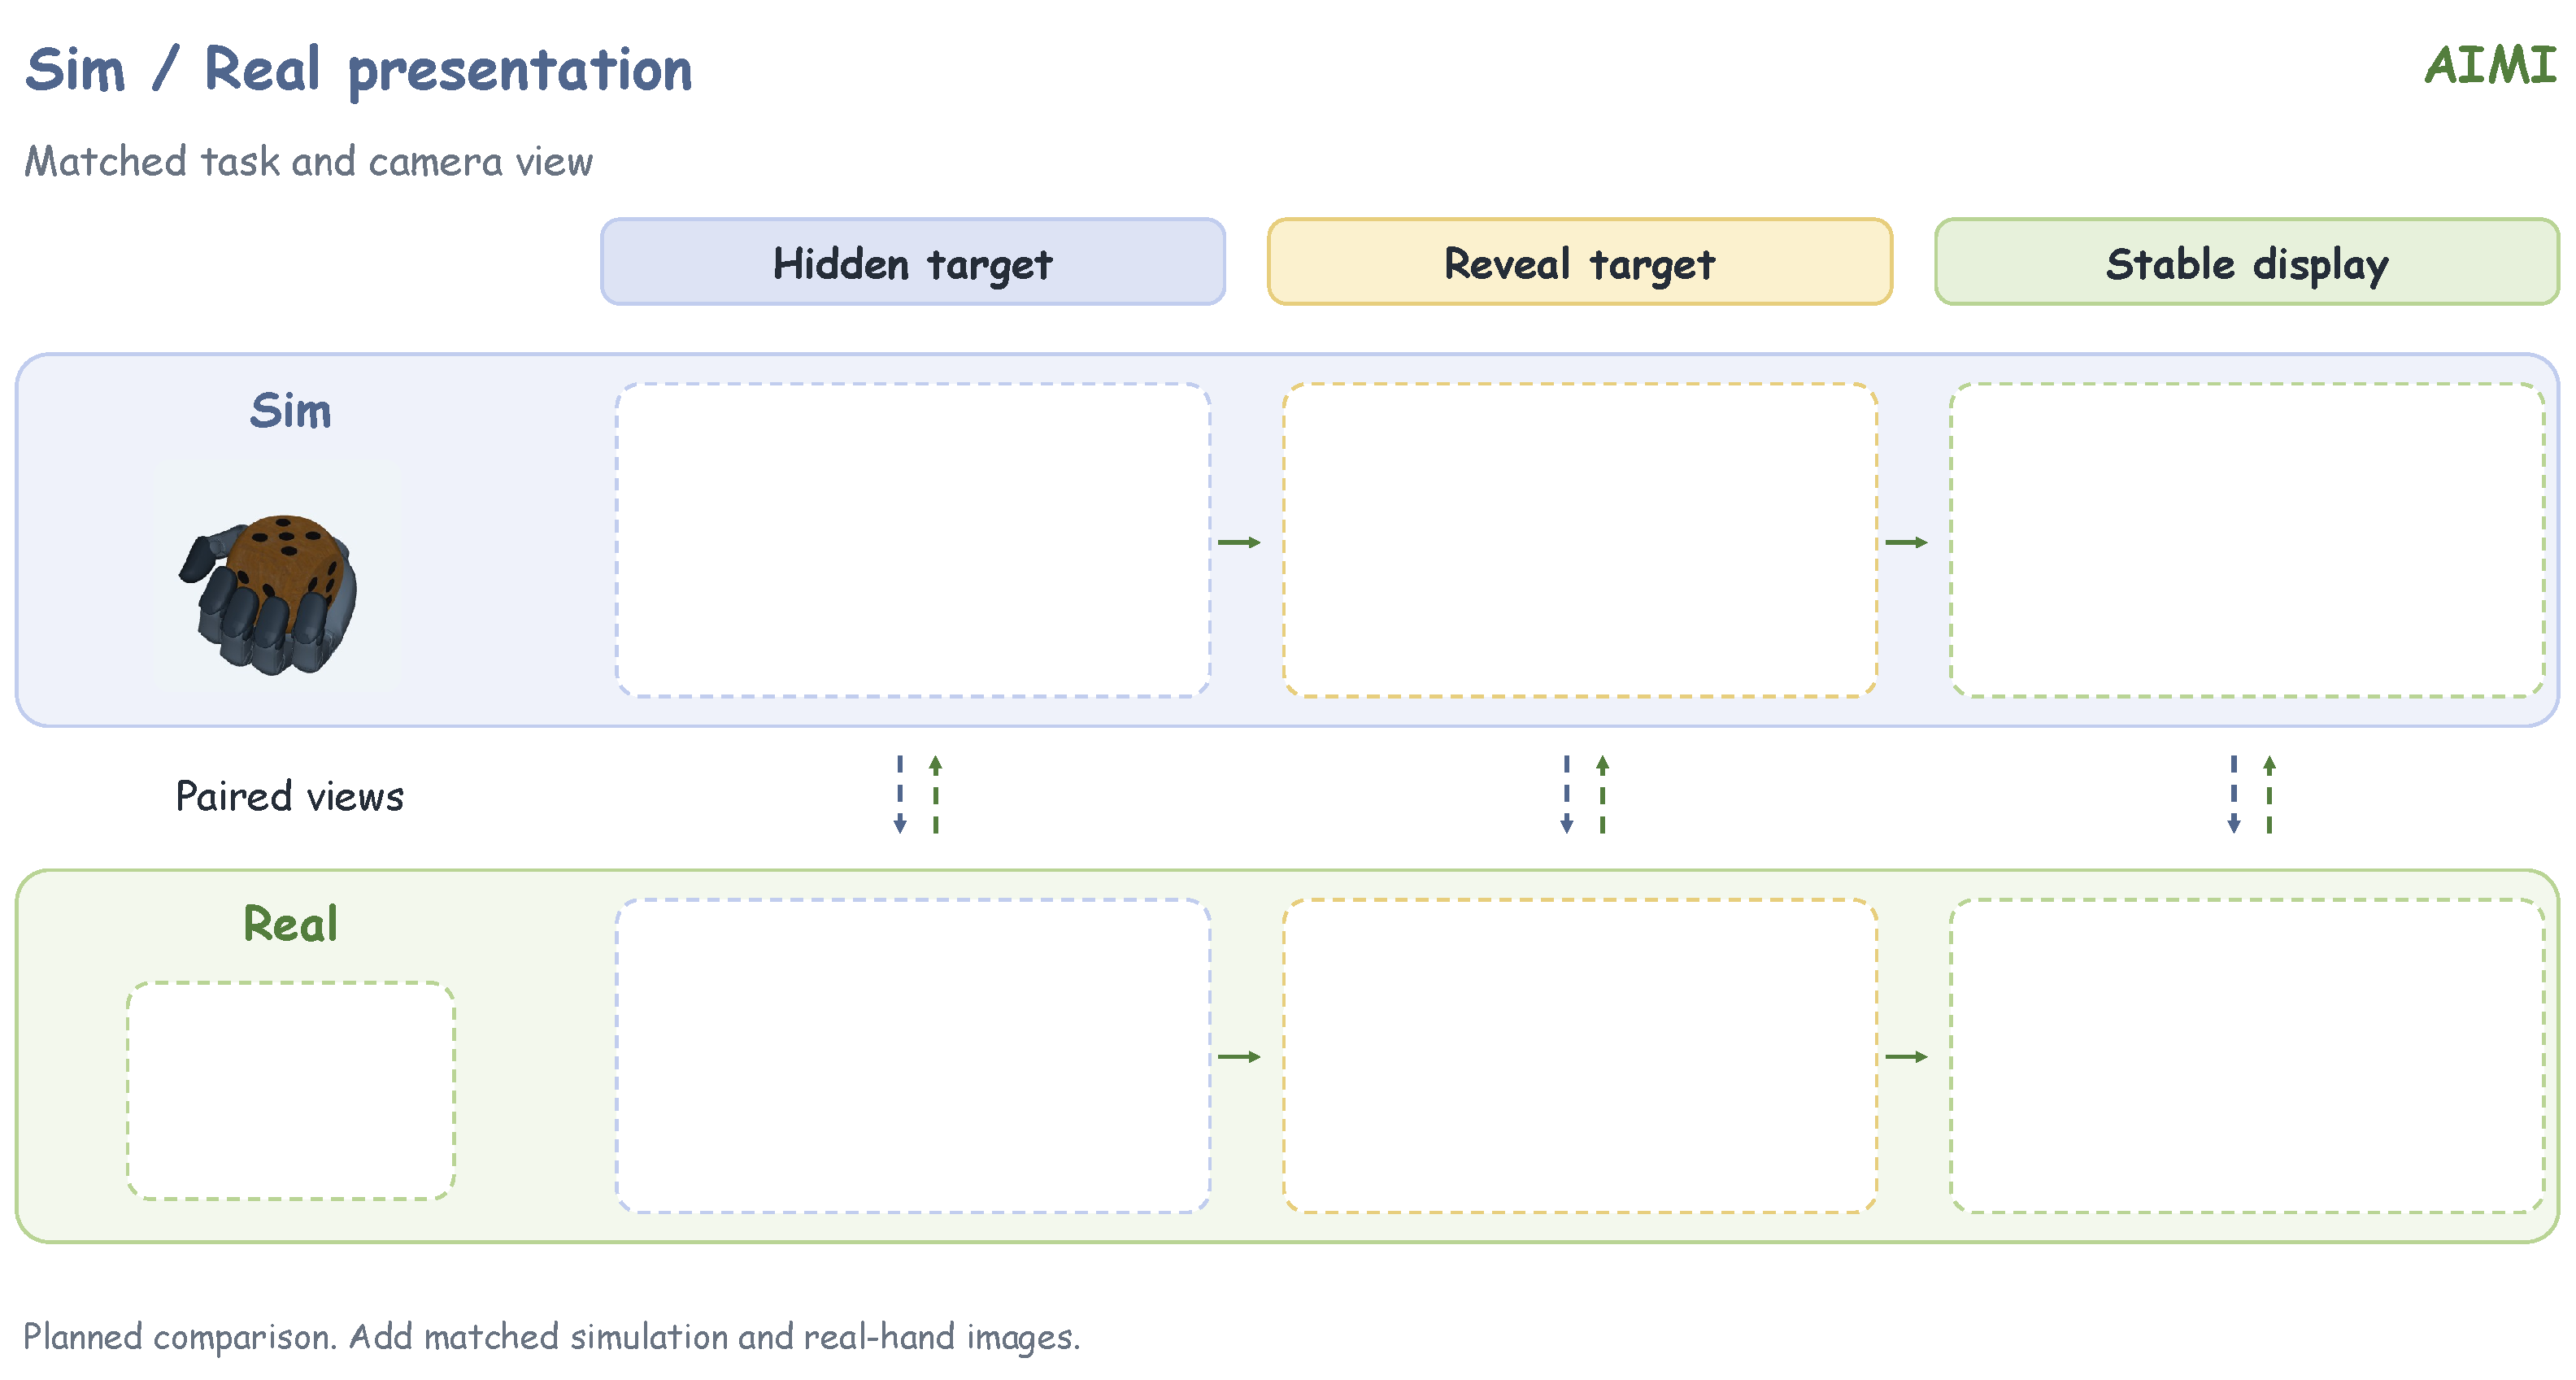
\includegraphics[width=0.95\textwidth]{figures/imported/aimi_sim_real.pdf}
\caption{\textbf{Planned simulation/physical presentation comparison.} The layout pairs hidden-target, reveal, and stable-display stages. The reference simulation crop is illustrative; the remaining simulation and physical-hand slots await matched observations. No real-robot outcome is represented.}
\label{fig:physical-panels}
\end{figure*}

\begin{figure*}[t]
\centering
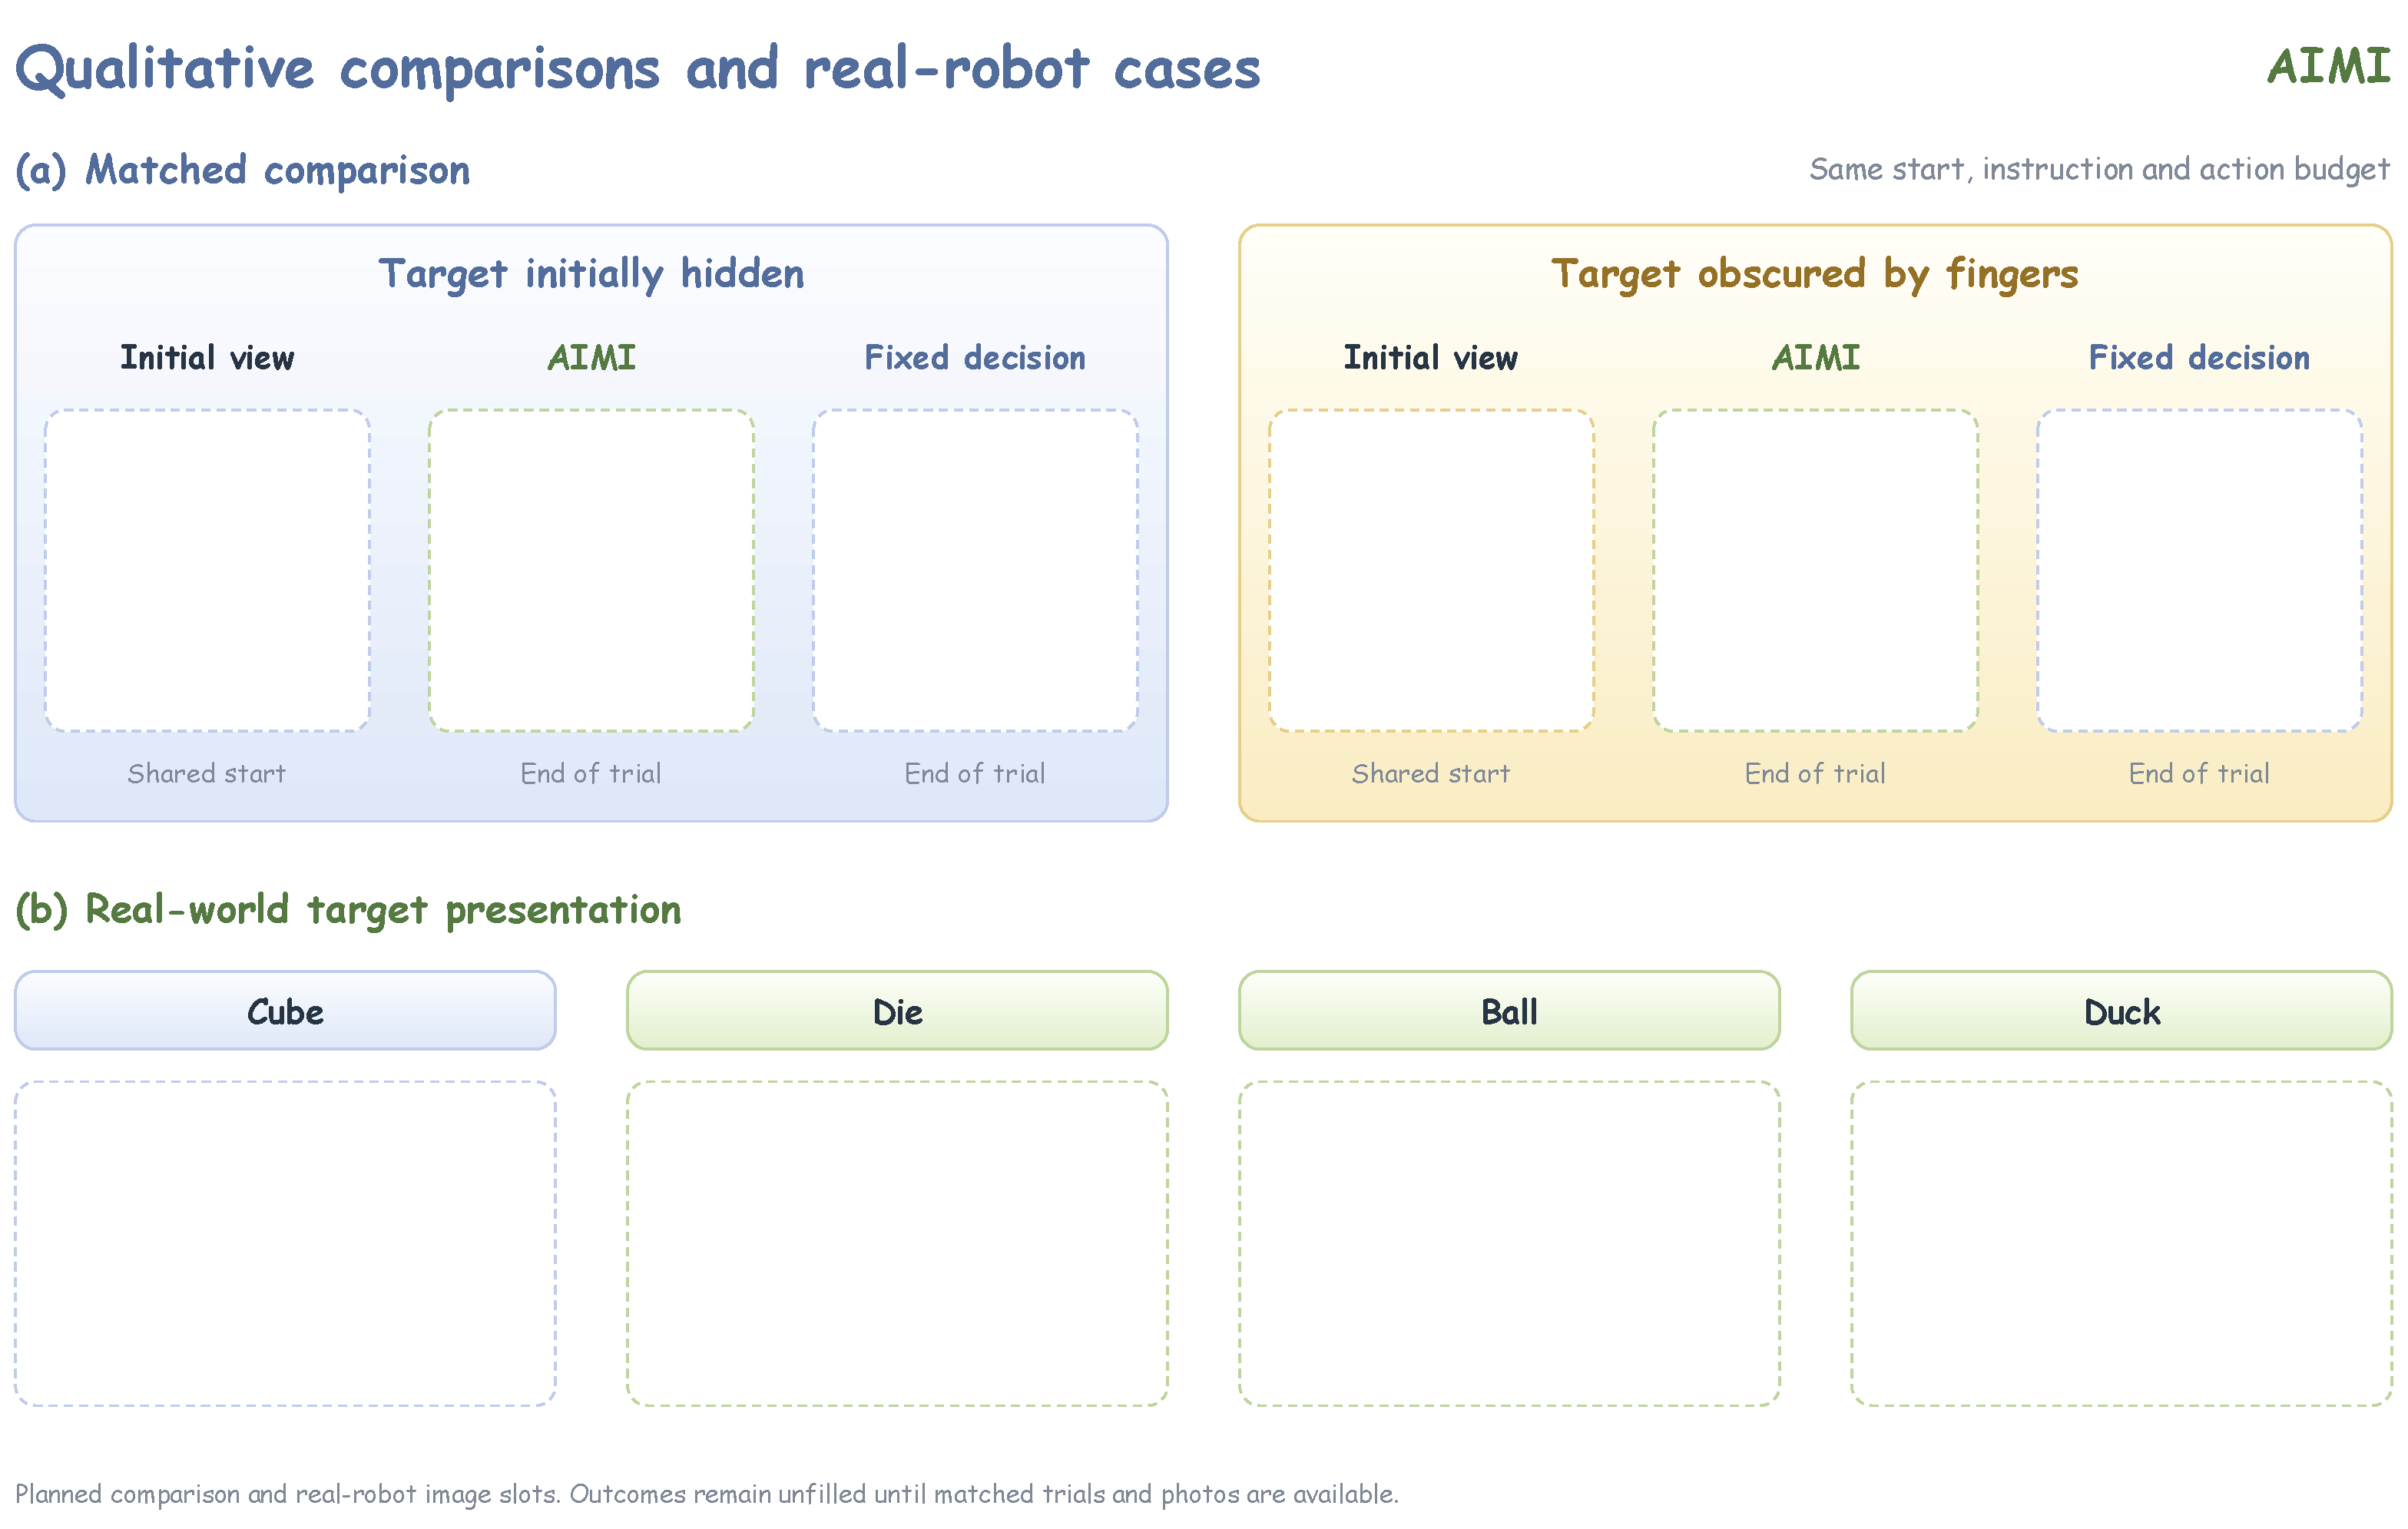
\includegraphics[width=0.95\textwidth]{figures/imported/aimi_real_cases.pdf}
\caption{\textbf{Planned qualitative comparison and real-robot cases.} Initial/end-state and physical-robot image slots remain placeholders until corresponding observations are available. No completed trial is represented.}
\label{fig:qualitative-real}
\end{figure*}

\section{Reproducibility}
The archived evidence retains outcomes, goals, stopping errors, service exclusions and latency for the audited cohorts. The three-seed controller aggregate is maintained separately from the historical trial records.

\TODO{Complete anonymous code and asset licenses.}
